\documentclass[10pt,a4paper]{article}
\usepackage[left=4cm,right=4cm,top=3.5cm,bottom=1.5cm]{geometry}
\usepackage[utf8]{inputenc}
\usepackage[english]{babel}
\usepackage[T1]{fontenc}
\usepackage{amsmath}
\usepackage{amsfonts}
\usepackage{amssymb}
\usepackage{lmodern}
\usepackage{siunitx}
\usepackage{fancyhdr}
\usepackage{enumerate}
\usepackage{mathtools}
\usepackage{float}
\usepackage{csquotes}
\usepackage{multicol}
\usepackage{lipsum}
\usepackage{tcolorbox}
\usepackage{enumitem}
\usepackage{varwidth}
\usepackage{todonotes}

% Setup SI units
\sisetup{locale=DE}
\sisetup{per-mode = symbol-or-fraction}
\sisetup{separate-uncertainty=true}
\DeclareSIUnit\year{a}
\DeclareSIUnit\clight{c}
 
 % Einbinden von Bildern
\usepackage{float}
\usepackage{graphicx, subfigure}	
	\graphicspath{{img/}}
\usepackage[skip=2pt]{caption}
 
% Abkürzungen
\usepackage{glossaries}
\newacronym{mpc}{MPC}{Model Predictive Control}
\newacronym{sos}{SOS}{Sum of Squares}
\newacronym{ocp}{OCP}{Optimal Control Problem}
\newacronym{sdp}{SDP}{Semidefinite Program}


 
% Being of document
%----------------------------------------------------------------------

% Defintions for the Document
\begin{document}
\pagestyle{fancy}
\lhead{University of Stuttgart}
\rhead{Institute of Flight Mechanics and Control}

% parskip
\setlength{\parindent}{0pt}

%----------------------------------------------------------------------

\begin{center}
	\LARGE{\textbf{Systems Theory Project Report}}\\[0.25em]
	\normalsize\textbf{Nonlinear Model Predictive Control Design}\\[0.25em]
	\normalsize{Elias Niepötter (3684096)}
\end{center}

\vskip 0.5cm

\begin{abstract}
	% \lipsum[1]
\end{abstract}

\vskip 0.5cm

% \begin{multicols}{2}

\section{Introduction}
The goal of the project is to combine the methods of \gls{sos} Programming and nonlinear \gls{mpc}.
Based on an exemplary nonlinear dynamical system an \gls{mpc} is designed in such a way that it acts outside a specified
region in the state space and drives it towards this region. The region is called \textit{terminal region}. Inside the
terminal region a linear controller takes over, this concept is called \textit{Dual Mode Control}. \gls{sos} methods are 
used to estimate the terminal region which is a \textit{region of attraction} of the closed loop dynamics of the linearly 
controlled system.
The report first introduces the basics of \gls{mpc} in \ref{sec:mpc}. Continuing with the concept of dual mode controller 
design focussing on \gls{sos} methods in \ref{sec:synTermCond}. Lastly, the methods presented are applied to the 
ball beam system. The results are shown and discussed in \ref{sec:example}. \todo{reformulate Introduction}

\section{Model Predictive Control}
\label{sec:mpc}
Model Predicitve Control is a flexible and powerful control strategy. It naturally handles nonlinearities constraints as
well as multiple inputs and outputs. The underlying idea is based on optimal control theory. \gls{mpc} is characterized by
two key features. First, an iterative online optimization is performed to compute the next control input. Second, at each 
instance of time an \gls{ocp} is solved, therefore the time horizon of the \gls{ocp} moves forward. \cite{nmpcBible}

\begin{figure}[h]
	\begin{center}
		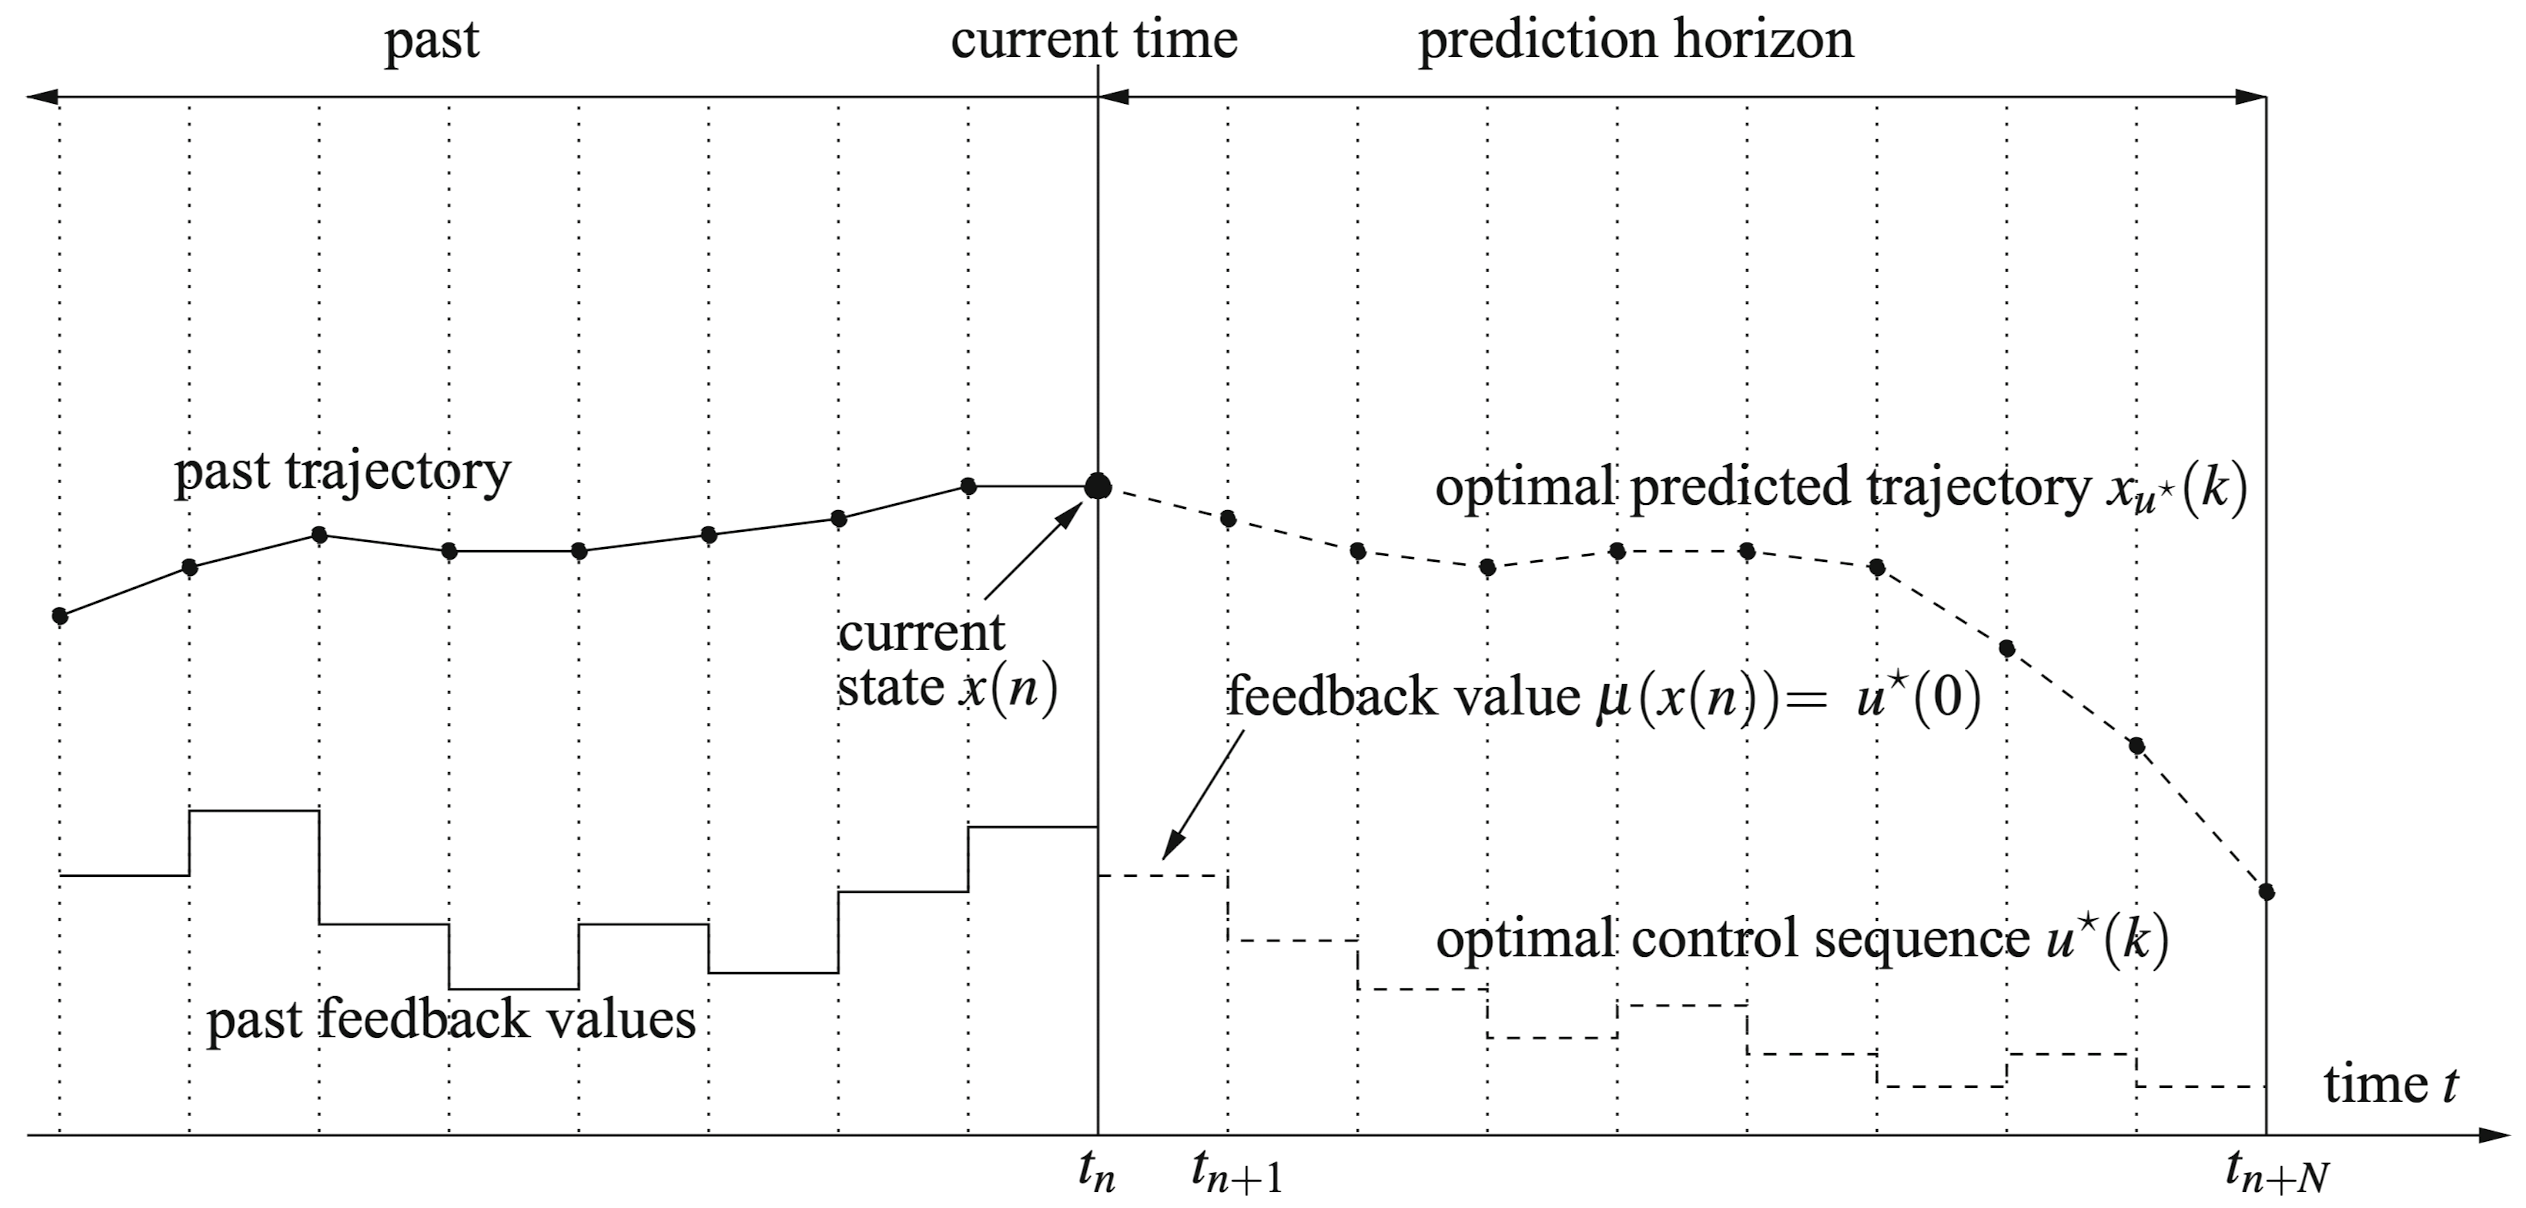
\includegraphics[width=0.8\textwidth]{img/nmpc_idea.png}
		\caption{Moving horizon and optimization of an MPC in discrete time \cite{nmpcBible}}
		\label{pic:nmpc_idea}
	\end{center}
\end{figure}

Figure \ref{pic:nmpc_idea} illustrates the two key feastures of \gls{mpc} in discrete time. At time instance $t_n$ 
the \gls{ocp} for the next $N$ time steps is solved. Given that the \gls{ocp} is feasible, the first optimal control
input $u^*_0$ is applied to the system. The system evolves to the next time instance $t_{n+1}$ and the process repeats.

\subsection{Problem Formulation}
The discrete time finite horizon optimal control problem can be formulated as follows:

\begin{align}
\label{eq:mpc_problem}
    \begin{array}{ll}
        \min\limits_{\nu} & E\left(x_{k+N \mid k}\right)+\sum_{i=k}^{k+N-1} F\left(x_{i \mid k}, u_{i \mid k}\right) \\[2em]
        \text { s.t. } & x_{i+1 \mid k}=f\left(x_{i \mid k}, u_{i \mid k}\right), \quad x_{k \mid k}=x_k\\
        & u_{i \mid k} \in \mathcal{U}, \quad i \in[k, k+N-1]\\
        & x_{i \mid k} \in \mathcal{X}, \quad i \in[k, k+N-1]\\
        & x_{k+N \mid k} \in \mathcal{E}
    \end{array}
\end{align}

where

\begin{equation}
\label{eq:mpc_costFunction}
    J\left(\nu, x_k\right)=\underbrace{E\left(x_{k+N \mid k}\right)}_{\text{terminal costs}} + \underbrace{\sum_{i=k}^{k+N-1} F\left(x_{i \mid k}, u_{i \mid k}\right)}_{\text{stage costs}}
\end{equation}

with $\mathcal{U}$ input constraints,  $\mathcal{X}$ state constraints and $\mathcal{E}$ terminal region/set as the constraining sets.
The \gls{ocp} is solved for the prediction horizon $N$, the initial condition $x_k$ at the current time step $t_k$, the dynamics
of the system given by $f\left(x_{i \mid k}, u_{i \mid k}\right)$ and the terminal state $x_{k+N \mid k}$. The cost function \eqref{eq:mpc_costFunction}
consists of the terminal costs at last time instance $t_N$ of the optimization and the stage costs for all other time instances starting from
the initial condition. The optimal control sequence is defined as

\begin{equation}
	\nu^* = [u_{k \mid k}^*, \dots , u_{k+N-1\mid k}^*]^T.
\end{equation}

The control input $\mu$ at each discrete time step $t_k$ is the first element of the optimal control sequence $\nu^*$

\begin{equation}
\mu(x(t_k)) \coloneqq \nu^*(0)
\end{equation}

See \cite{nmpcBible} and \cite{RaffAllgoewer} for details on the formulation of the \gls{ocp} resp. the \gls{mpc} formulation.

\subsection{Terminal Conditions for MPCs}
The shown \gls{mpc} includes terminal conditions. These conditions are part of the design of the \gls{mpc} and are used to
guarantee certain stability properties of the closed loop system. The followong Theorem connects terminal conditions and
stability of the closed loop system. \cite{RaffAllgoewer}

\begin{tcolorbox}[colback=gray!20, colframe=gray!80,title=Theorem 1,arc=0.0mm]
The closed loop system is asymptotically stable if the optimal control problem is feasible at the first time instant and
the following assumptions are satisfied for a terminal cost $E$, a terminal region $\mathcal{E}$, and a locally stabilizing
control law $u_{k}=\varphi\left(x_{k}\right)$:

[A1] $E\left(x_{k}\right)>0, \forall x_{k} \in \mathbb{R}^{n} \backslash\{0\}$

[A2]  $\mathcal{E} \subseteq \mathcal{X}, 0 \in \mathcal{E}$

[A3] $\varphi\left(x_{k}\right) \in \mathcal{U}, \forall x_{k} \in \mathcal{E}$

[A4] $f\left(x_{k}, \varphi\left(x_{k}\right)\right) \in \mathcal{E}, \forall x_{k} \in \mathcal{E}$

[A5] $E\left(f\left(x_{k}, \varphi\left(x_{k}\right)\right)\right)-E\left(x_{k}\right) \leq-F\left(x_{k}, \varphi\left(x_{k}\right)\right), \forall x_{k} \in \mathcal{E}$.
\end{tcolorbox}

Several approaches based on Theorem 1 exist to ensure closed loop stability. Those investigated in this work are the following:\\

\textbf{Zero Terminal State Constraint}\\
The idea is to use $E(x_k) = 0$, $\mathcal{E} = \{ 0 \}$ and $\varphi(x_{k}) = 0$. No linear controller is used.
The stability of the \gls{mpc} is guaranteed through $x_{k+N \mid k} = 0$. When assuming an equlibrium at the
origin of the system, this ensures stability at the last step of the \gls{ocp}.\\

\textbf{Terminal Region}\\
No terminal costs are used, but a terminal region $\mathcal{E} = \{x_k \in \mathbb{R}^n \mid x_k^TPx_k \leq \alpha \}$
is choosen as well as a locally stabilizing linear controller $\varphi(x_{k}) = K x_k$. This approach is also
\textit{dual mode control}.\\

\textbf{Terminal Region and Terminal Cost}\\
The so-called quasi-infinite horizon \gls{mpc} uses a terminal region $\mathcal{E} = \{x_k \in \mathbb{R}^n \mid x_k^TPx_k \leq \alpha \}$
and a terminal cost $E(x_k) = x_k^T P x_k$ as well as locally stabilizing linear controller $\varphi(x_{k}) = K x_k$.
The terminal cost $E$, terminal region $\mathcal{E}$ and locally stabilizing linear controller $\varphi(x_{k})$ are 
calculated off-line. The procedure is described in section \ref{sec:synTermCond}.


\subsection{Variations of \gls{mpc}}
There are several variations of the \gls{mpc} formulation. Two important distinctions have to be made regarding the length
of the prediction horiton. One differentiate between \textit{finite} and \textit{infinite} horizon optimal control. presented
above is the finite horizon \gls{mpc}. The infinite horizon \gls{mpc}, as the name implies, has an infinite prediction horizon
$N \rightarrow \infty$. It can be shown that the inifinte horizon \gls{mpc} asymptotically stabilizes the system, without need
of any terminal conditions. Hence the name \textit{quasi-infinite horizon} is motivated by this property.
Furthermore, it should be differentiated between \textit{stabilizing} and \textit{tracking} \gls{mpc}. The stabilizing \gls{mpc}
is used to stabilize the system around an equilibrium point. The tracking \gls{mpc} is used to follow
a reference trajectory as good as possible. For the stabilizing \gls{mpc} the reference can assumed by constant zero, when the 
system is stable around the origin. Given the definitions above, it is possible to introduce the tracking \gls{mpc} by utilizing
the difference, or error, of the current state to the reference $e_k = x_k - x_{\text{ref},k}$ as a new state. In other words,
the tracking \gls{mpc} is a stabilizing \gls{mpc} for the error dynamics of the system. Tracking \gls{mpc} won't be considered in
the follwing. For more details see \cite{nmpcBible}. 


\section{Synthesis of Terminal Conditions}
\label{sec:synTermCond}
Followed by the introduction of terminal conditions and their application in \gls{mpc}, the synthesis of terminal cost $E$, the
terminal region $\mathcal{E}$ and the locally stabilizing linear controller $\varphi(x_{k})$ is presented. The procedures are based
on \cite{CHEN19981205}. This section draws the connection to \gls{sos} programming. The procedure is as follows:\\

\textit{Step 1.} Solve the linear control problem based on the jacobian linearization of the nonlinear system and obtain the feedback
matrix $K$.\\

\textit{Step 2.} Choose a constant $\kappa \in [0,\infty)$ satisfying
\begin{equation}
	\kappa < -\lambda_{\text{max}}(A_K)
\end{equation}

where $A_K \coloneqq A + BK$ expressing the closed loop dynamics of the linearized and locally controlled system. The operator
$\lambda_{\text{max}}(\cdot)$ denotes the maximum eigenvalue of a matrix. Furthermore, solve the lyapunov equation

\begin{equation}
	\left(A_K+\kappa I\right)^{\mathrm{T}} P+P\left(A_K+\kappa I\right)=-Q^*
\end{equation}

where $Q^* = Q + K^T R K \in \mathbb{R}^{n \times n}$ itself is positive definite and symmetric. The obtained matrix $P$ is 
positive definite and symmetric. The matrices $Q$ and $R$ might be used for \textit{Step 1} to obatain the linear feedback
matrix $K$ based on LQ-regulators.\\

\textit{Step 3.} Find the largest possible $\alpha_1$ s.t $Kx \in \mathcal{U} \quad \forall x \in \Omega_{\alpha_1}$.\\

\textit{Step 4.} Find the largest possible $\alpha \in (0,\alpha_1]$ s.t. $\{x_k \in \mathbb{R}^n \mid x_k^TPx_k \leq \alpha \}$ is an 
inner approximation of the region of attraction of the closed loop dynamics of the linearly controlled system.


\subsection{Lyapunov's second method for stability} \todo{Source?}
In order to estimate a region of attraction, Lyapunov's second method for stability is used. The method makes use of the concept of \textit{dissipativity}.
Consider the dynamical system $f(x) = \dot{x}$ and a \textit{storage function} $V: \mathbb{R}^n \rightarrow \mathbb{R}$ where $\mathbb{R}^n$ denotes the state space.
The system is asymptotically stable in the sense of Lyapunov if the following conditions hold:
\begin{align}
	V(x) &= 0 \text{ if and only if } x=0\\
	V(x) &> 0 \text{ if and only if } x\neq0\\
	\dot{V}(x) &= \nabla V \cdot f(x) < 0 \quad \forall x \neq 0
\end{align}
In that case, $V(x)$ is calles a \textit{Lyapunov function}. Note that these conditions are not sufficient to prove global asymptotical stability.
For that to be the case, $V(x)$ also has to be radially unbounded.


\subsection{\gls{sos} Programming \cite{cunis_loureiro2023}}
\gls{sos} programming is used to \textit{verify} wether a given, potentially multivariate, polynomial $p(x) \in \mathbb{R}[x]$, where $\mathbb{R}[x]$ denotes
the ring of polynomial in $x \in \mathbb{R}^n$ with real coefficients, is a sum-of-squares polynomial. A polynomial $p \in \mathbb{R}^n$ is sum-of-squares if
there exists $q_1, \dots, q_m$ s.t.

\begin{equation}
	p(x)=\sum_{i=1}^m q_i^2(x)
\end{equation}

The set of \gls{sos} polynomials will be denoted by $\Sigma[x]$. If a polynomial is sum-of-squares, it is also a nonnegativ polynomial $p(x) \geq 0$.
Subsequently, if we want to proof wether a polynomial is nonnegative or not, we can now relax this problem to the question, wether the the polynomial
is sum-of-squares or not. The advantage of this relaxation over the orginal problem is that solving the problem to verify if a polynomial is 
sum-of-squares can be done in polynomial time. Proofing if a polynomial is nonnegative is a NP-hard problem. The verification on whether a polynomial
is sum-of-squares or not is done by solving a \gls{sdp}.\\

\textbf{Lemma 1}. Let $p(x) \in \mathbb{R}[x]$ be a polynomial of degree $d$. Then, $p(x) \in \Sigma[x]$ if and only if there exists a symmetric
matrix $Q \in \mathbb{S}^l$ being positive semidefinite (all eigenvalues of $Q$ are nonnegative) such that
\begin{equation}
	p(x)=z(x)^{\top} Q z(x)
\end{equation}
for some monomial vector $z(x) \in \mathbb{R}[x]^l$ with $\operatorname{deg}(z(x)) \leq \frac{d}{2}$.\\

Using Lemma 1, we further relaxed the problem of verifying if a polynomial is sum-of-squares to the problem of finding a positive semidefinite matrix $Q$.
This task is done via a \gls{sdp}. \todo{More details in SDP?}\\


The following procedure, called \textit{Generalized S-procedure}, is used to solve the set containment problem:

\begin{tcolorbox}[colback=gray!20, colframe=gray!80,title=Generalized S-procedure \cite{cunis_loureiro2023},arc=0.2mm]        
Given $h, f_0, \ldots, f_r \in \mathbb{R}[x]$, if there exist $p \in \mathbb{R}[x]$, and $s_1, \ldots, s_f \in \Sigma[x]$ s.t.
\begin{equation}
	\text { ph }-\sum_{j=1}^r s_j f_j+f_0 \in \Sigma[x]
\end{equation}
then the following set containment holds:
\begin{equation}
	\left\{x \in \mathbb{R}^n \mid h(x)=0, f_1(x) \geq 0, \ldots, f_r(x) \geq 0\right\} \subseteq\left\{x \in \mathbb{R}^n \mid f_0(x) \geq 0\right\}
\end{equation}
\end{tcolorbox}


\subsection{Sublevel set optimization}
In \textit{Step 3} and \textit{4} one tries to find the largest sublevel set of a given function satisfying certain constraints. These optimization problems
can be formulated to one single problem. The idea is to setup a nonlinear root search for the parameter $\alpha$. An iterative 
algorithm, e.g. a bisection algorithm \todo{short description of the algorithm}, is used to maximize the parameter. The problem can be formulated as follows:

\begin{equation}
\label{eq:sos_problem}
\max\limits_{\alpha} \quad \text{V}\left(\{x_k \in \mathbb{R}^n \mid x_k^TPx_k \leq \alpha \}\right)
\end{equation}

The resulting constraints for the optimiztion are
\todo{Finish full problem formulation}
\begin{align}
	s_{i} &\in \Sigma[x]\\
	-s_{i}(-x^TPx + \alpha_1) + (Kx + u_{\text{max},i}) &\in \Sigma[x]\\
	-s_{N_u +i}(-x^TPx + \alpha_1) + (-Kx - u_{\text{min},i}) &\in \Sigma[x]
\end{align}










\pagebreak
\section{Exemplary Application}
\label{sec:example}
\todo{Implementation details? Multiple Shooting?}
Based on an exemplary system a \gls{mpc} with terminal conditions is designed using the procedures described above. 


\subsection{Setup}
The exemplary system is the ball beam system.
It consists of a ball rolling on a beam. The beams angle is controlled by a motor. Gravity acting on the ball accelerates it accoding to the angle of the beam.
The system is described by the following equations of motion:

\begin{equation}
    0 = \left(\frac{J}{R^2} + m\right)\ddot{r} + mg\sin(\alpha) = - mr\dot{\alpha}^2
\end{equation}


States are chosen as
\begin{equation}
	x = \begin{bmatrix} r & \dot{r} & \alpha & \dot{\alpha} \end{bmatrix}^T
\end{equation}

and the input as
\begin{equation}
	u = \ddot{\alpha}
\end{equation}


\begin{align*}
    \dot{x} = f(x,u) = \begin{bmatrix}
        x_2 \\
        m x_1 x_4^2 - m g \left(\frac{x_3^5}{120} - \frac{x_3^3}{6} + x_3\right) \cdot k \\
        x_4 \\
        u
    \end{bmatrix}
\end{align*}

Note that the $\sin()$ term is approximated by a Taylor series epansion of degree five in order to obtain a polynomial system. The constant $k$ combines 
the physical parameters of the system. Table \ref{tbl:controler} gives an overview of the different \gls{mpc} controler setups used.

\renewcommand{\arraystretch}{1.25}
\begin{table}[ht]
    \centering
    \captionsetup{skip=0.25cm}
    \caption{overview of additional terms}
    \label{tbl:controler}
    \begin{tabular}{|p{2cm}|p{4cm}|p{5.5cm}|}
        \hline
        \textbf{Controller} & \textbf{Name} &  \textbf{Explanation}\\
        \hline
        QIH & Quasi-Inifnite Horizon & terminal region + costs\\
        \hline
        TR & Terminal Region & just terminal region\\
        \hline
        TC & Terminal Constraint & terminal constraint to end in equilibrium\\
        \hline
        NTC & No Terminal Conditions & no terminal conditions at all\\
        \hline
    \end{tabular}
\end{table}

The TC and NTC controller consists just of the \gls{mpc}. The QIH and TR controller have linear controller which takes over as soon as they enter the terminal region.
The time step for the closed loop simulation is set to $\Delta t_{\text{cl}} = \SI{0.01}{\second}$.  The time step for the \gls{mpc} is set to
$\Delta t_{\text{mpc}} = \SI{0.05}{\second}$. The prediction horizon is set to $N = \SI{1}{\second}$. No noise is added to the states and the true
model is known. The stage costs are chosen to

\begin{equation}
	F\left(x_{i \mid k}, u_{i \mid k}\right) = \frac{1}{2} \lVert x_{i \mid k} \rVert_2 + \frac{1}{2} \lVert u_{i \mid k} \rVert_2.
\end{equation}


\subsection{Results}
Figure \ref{pic:bb_state_space} to \ref{pic:bb_time_u} show the results of the simulations. Most obvious is the rather poor performance of the NTC controller.
It has highest excitations especially in state $x_3 = \alpha$ and $x_4 = \dot{\alpha}$ (see fig. \ref{pic:bb_state_space}).

\begin{figure}[h]
	\begin{center}
		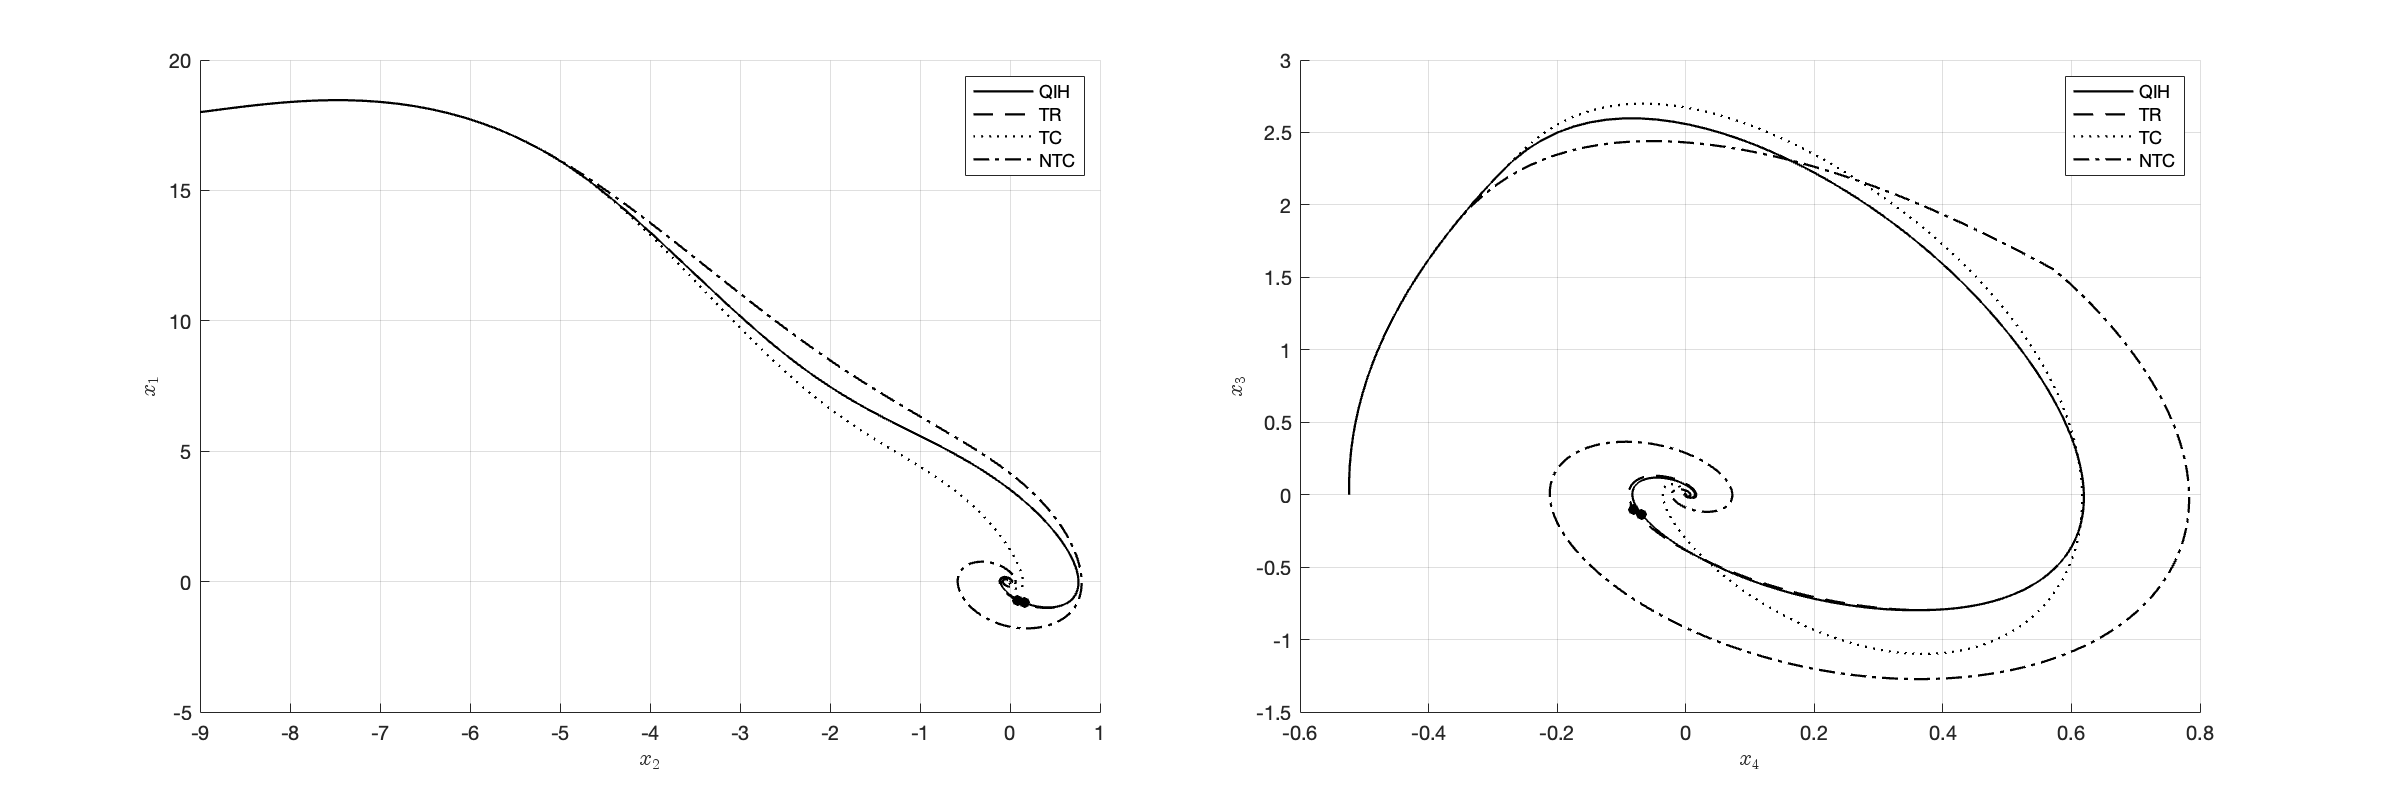
\includegraphics[width=\textwidth]{img/bb_states.png}
		\caption{state space trajectories for defined control setups}
		\label{pic:bb_state_space}
	\end{center}
\end{figure}

Compared to the other controllers, the NTC controller also takes longest to fully converge to the equilibrium. However, the NTC controller is still able to
stabilize the system. The most performant controller is the TC controller. It has the largest occuring input to the systems  and the fastest covergence.
This result was to expect, because the TC controller (the \gls{mpc}) has to bring the system to the equilibrium in the given time horizon of $\SI{1}{\second}$. 

\begin{figure}[h]
	\begin{center}
		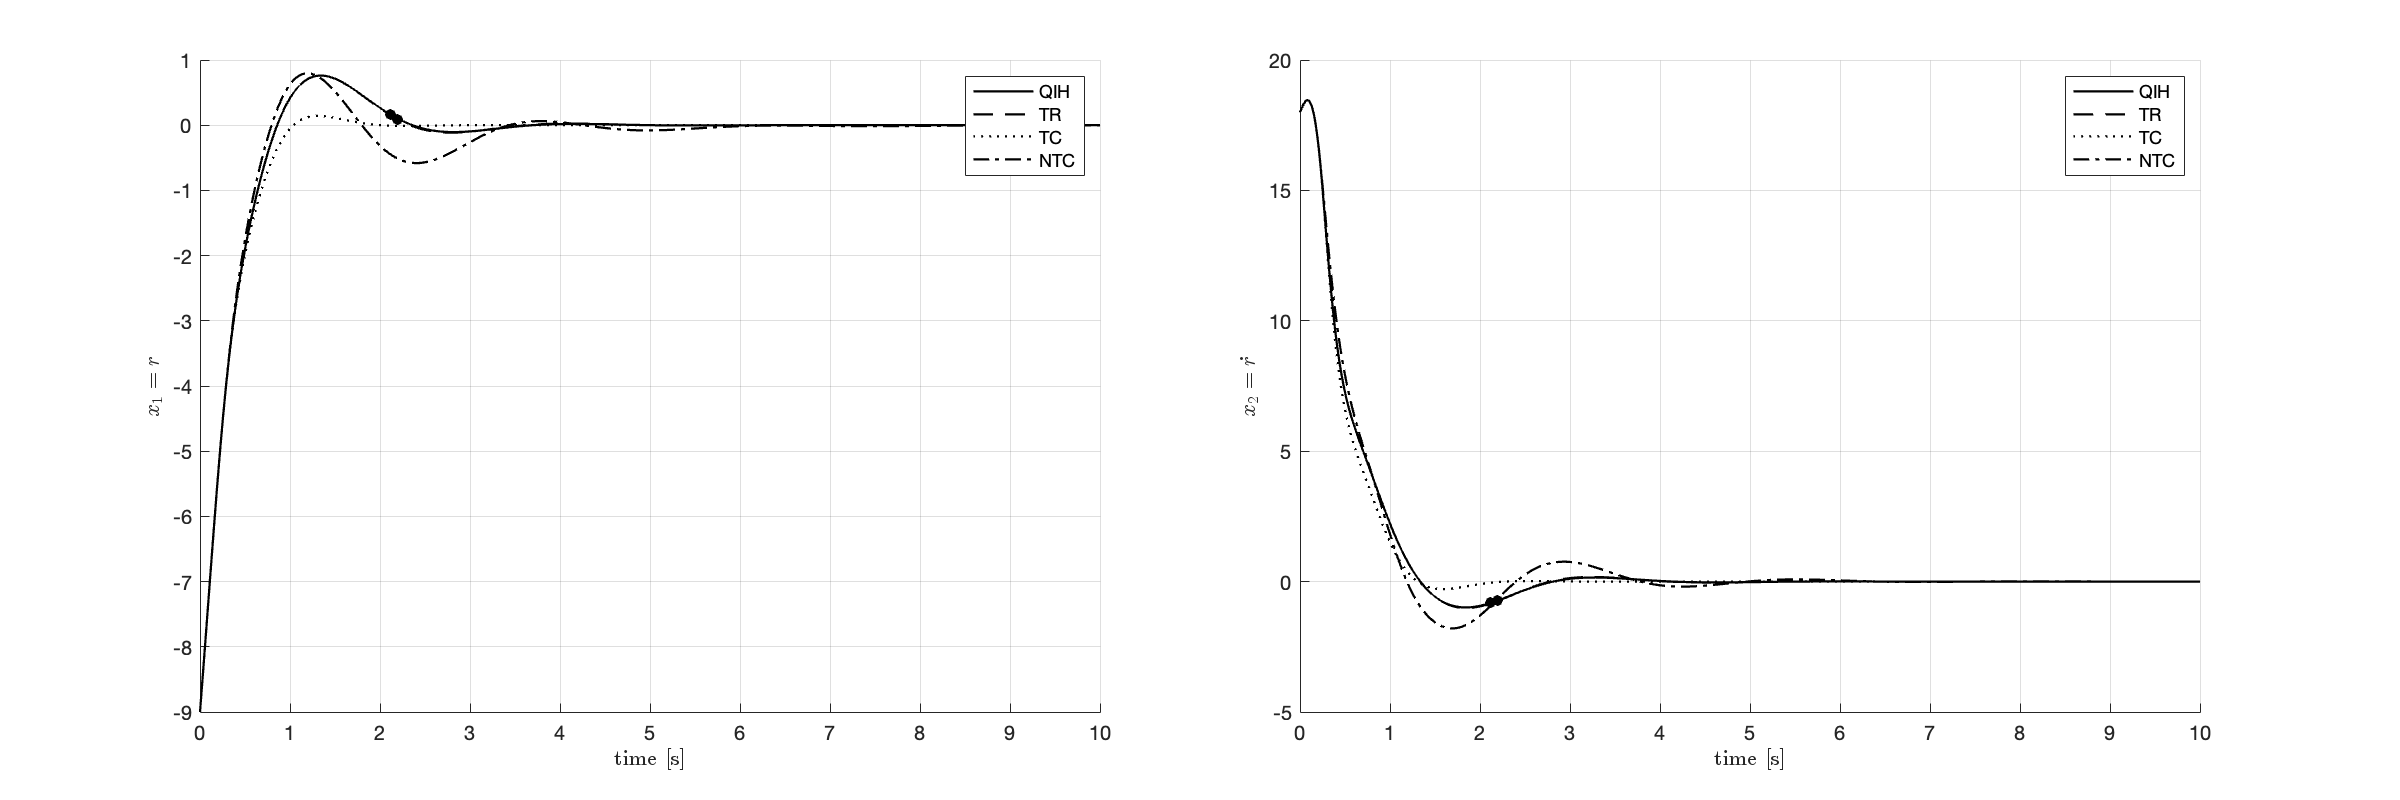
\includegraphics[width=\textwidth]{img/bb_time_x1x2.png}
		\caption{trajectories for states $x_1$ and $x_2$}
		\label{pic:bb_time_x1x2}
	\end{center}
\end{figure}

\begin{figure}[h]
	\begin{center}
		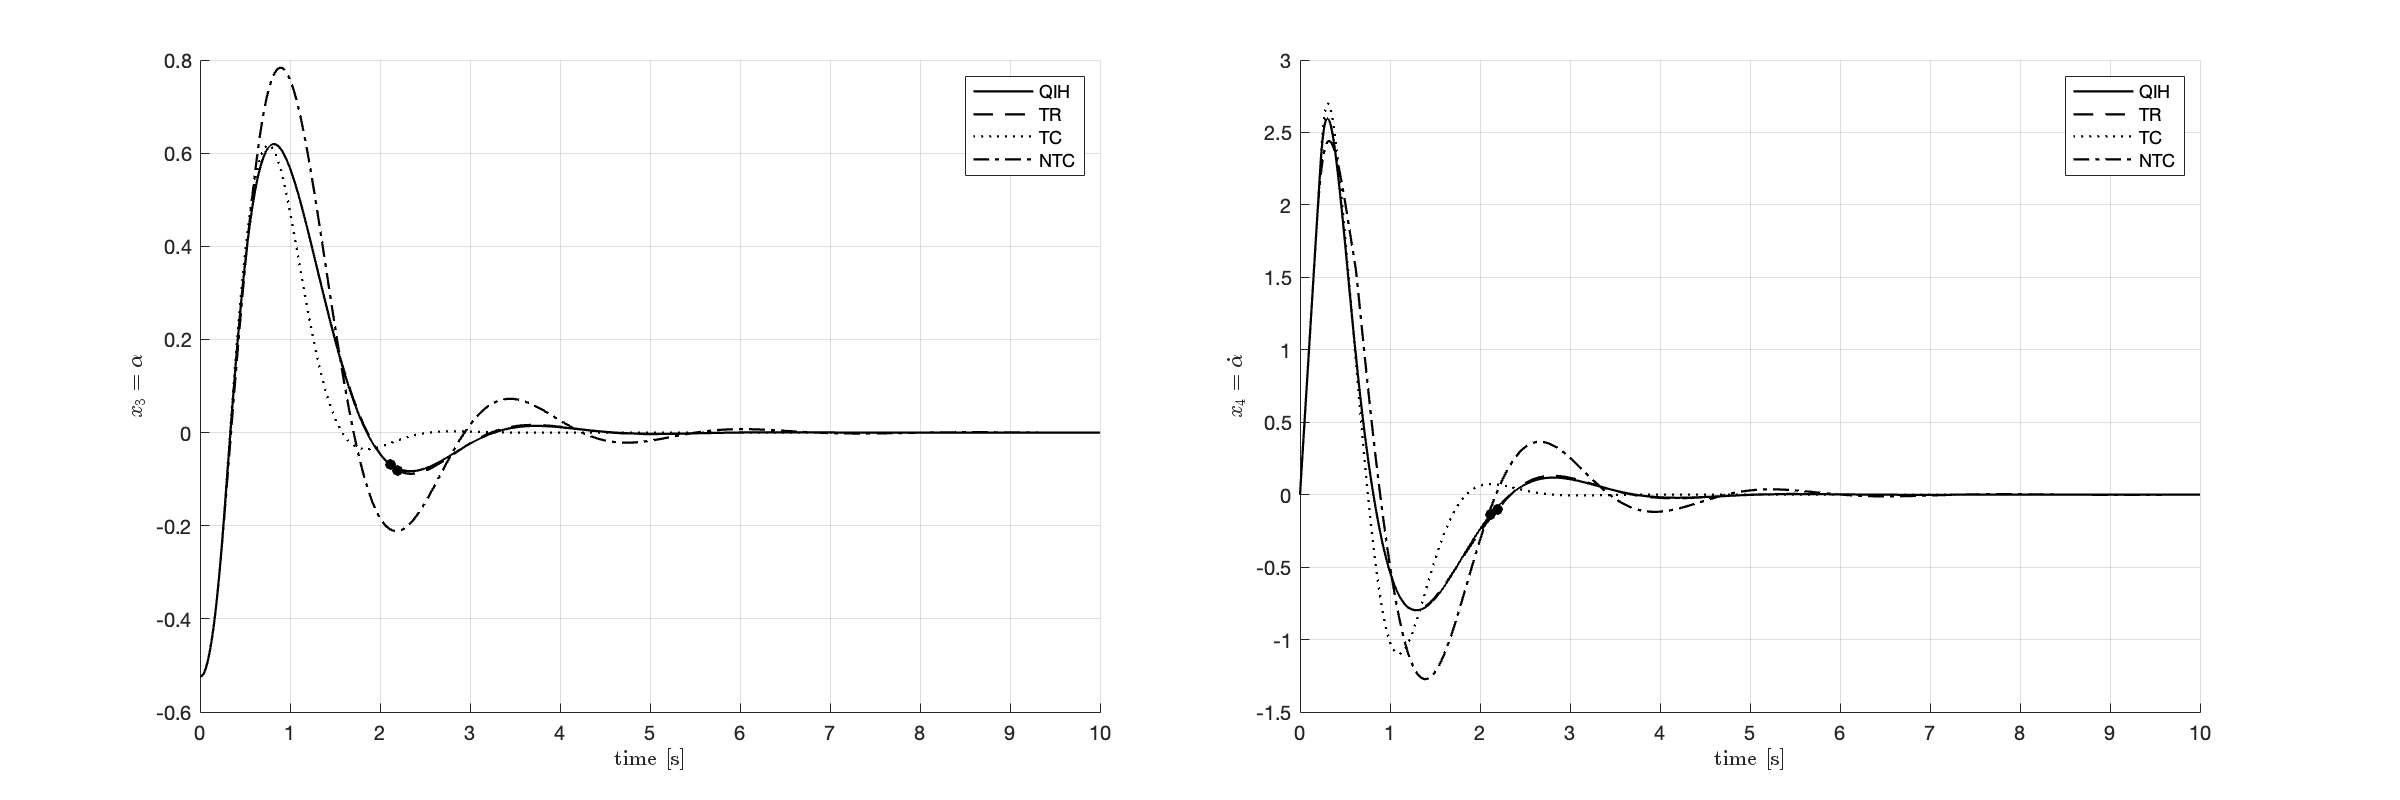
\includegraphics[width=\textwidth]{img/bb_time_x3x4.png}
		\caption{trajectories for states $x_3$ and $x_4$}
		\label{pic:bb_time_x3x4}
	\end{center}
\end{figure}

The QIH controller and the TR controller show similar performance. Compared to the NTC and TC controller, their perofemance is in between. With their respective 
design approach in mind, this result was also to expect. The \gls{mpc} of the QIH and TR controller just has to get the system into the terminal region.

\begin{figure}[h]
	\begin{center}
		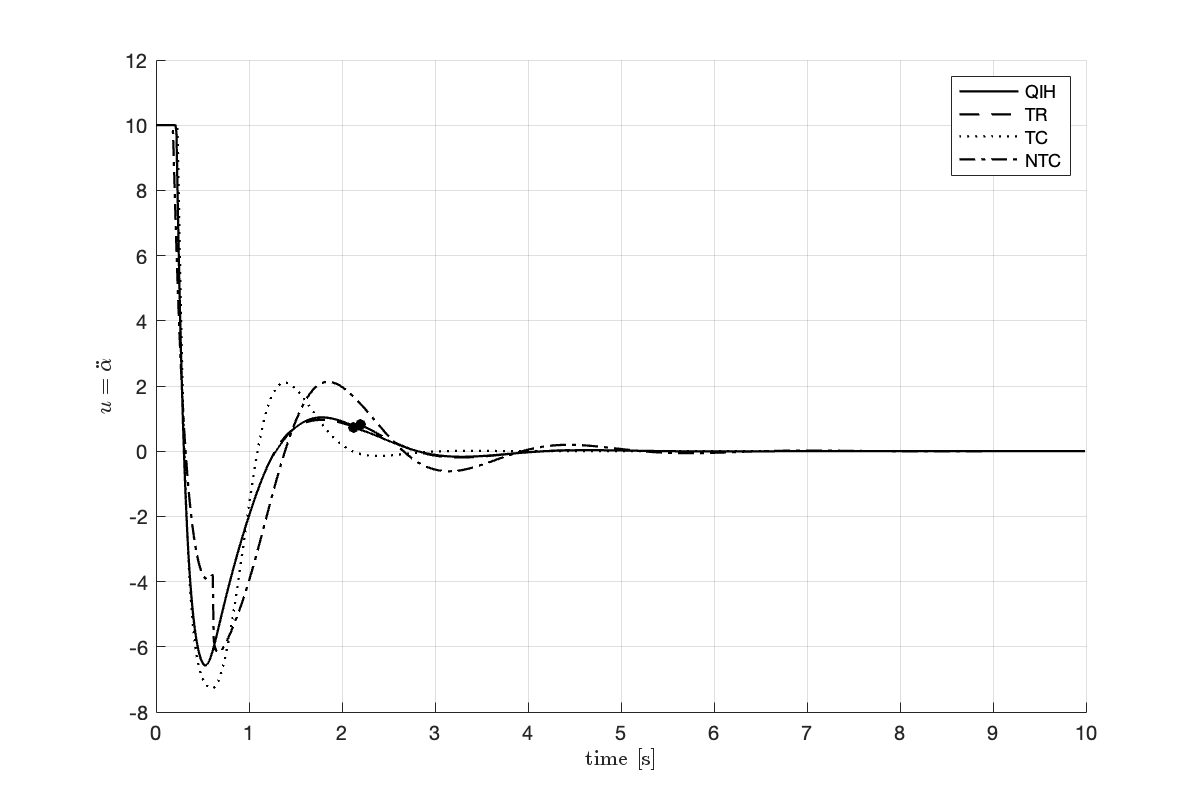
\includegraphics[width=\textwidth]{img/bb_time_u.png}
		\caption{trajectories for input $u$}
		\label{pic:bb_time_u}
	\end{center}
\end{figure}

Figure \ref{pic:bb_time_u} shows that the QIH and TR controller have overall the lowest input to the system. Furthermore, the QIH and TR controller have very similar
trajectories and behavior. The terminal costs don't seem to have an significant impact for this specific example. The black dots in all result figures show the
switching point of the dual mode controller, so the point from where on the linear controller controls the system. The QIH controller enters the terminal region
slightly earlier than the TR controller. 


\section{Conclusion \& Outlook}
\label{sec:conclusion}

\todo{Briefly introduce the other usage of SOS covered by Allgoewer}






\pagebreak
\bibliography{references}
\bibliographystyle{plain}

\pagebreak
\listoftodos

% \end{multicols}
\end{document}